\documentclass[bachelor]{thesis-uestc}
\usepackage{indentfirst}
\usepackage{amssymb, amsmath}
\usepackage{graphicx, subfigure}
\usepackage{algorithm, algorithmic, float}
% 没有使用thesis-uestc的算法模板, 需将thesis-uestc中的相关内容注释掉, 避免冲突
\usepackage{listings}
\usepackage{fancyhdr}
\usepackage{booktabs}

%\begin{figure}[htbp]
%	\centering\includegraphics[height=10cm]{images/pic.png}
%	\caption{caption_name}
%	\label{fig:pic}
%\end{figure}

%\begin{lstlisting}[language=C++, basicstyle=\ttfamily\tiny, numbers=left, numberstyle=\tiny, keywordstyle=\color{blue!70}, commentstyle=\color{red!50!green!50!blue!50}, frame=shadowbox, rulesepcolor=\color{red!20!green!20!blue!20}]

%\end{lstlisting}

% ----------------------------------------- Document -----------------------------------------

\begin{document}

% ----------------------------------------- 目录 -----------------------------------------
\thesistableofcontents

% ----------------------------------------- 正文 -----------------------------------------
\thesischapterexordium % 第一章 课题背景

\chapter{相关技术介绍}

\chapter{关键技术研究}

\chapter{系统实现}
\section{shellcode设计}
shellcode要实现的功能是:以字符串``cmd''为参数,调用C库的system()函数启动一个shell。

\subsection{获取C库的加载基地址}
在安装了vs2013的win7 x64或x64操作系统中,Release版本的win32程序使用的C库是msvcr120.dll,该DLL在程序加载时被映射到进程的地址空间内,因此需要获取该DLL模块的加载基地址。
win32程序进程的地址空间中,FS:[0x30]处保存着一个指向进程环境块(PEB)的指针。PEB结构如下:

\begin{lstlisting}[language=C++, basicstyle=\ttfamily\tiny, numbers=left, numberstyle=\tiny, keywordstyle=\color{blue!70}, commentstyle=\color{red!50!green!50!blue!50}, frame=shadowbox, rulesepcolor=\color{red!20!green!20!blue!20}]
typedef struct _PEB {
	BYTE                          Reserved1[2];
	BYTE                          BeingDebugged;
	BYTE                          Reserved2[1];
	PVOID                         Reserved3[2];
	PPEB_LDR_DATA                 Ldr; // +0x0c 
	PRTL_USER_PROCESS_PARAMETERS  ProcessParameters;
	PVOID                         Reserved4[3];
	PVOID                         AtlThunkSListPtr;
	PVOID                         Reserved5;
	ULONG                         Reserved6;
	PVOID                         Reserved7;
	ULONG                         Reserved8;
	ULONG                         AtlThunkSListPtr32;
	PVOID                         Reserved9[45];
	BYTE                          Reserved10[96];
	PPS_POST_PROCESS_INIT_ROUTINE PostProcessInitRoutine;
	BYTE                          Reserved11[128];
	PVOID                         Reserved12[1];
	ULONG                         SessionId;
} PEB, *PPEB
\end{lstlisting}

PEB结构体偏移+0x0c处是一个指向PEB\_LDR\_DATA结构的指针。PEB\_LDR\_DATA结构如下:

\begin{lstlisting}[language=C++, basicstyle=\ttfamily\tiny, numbers=left, numberstyle=\tiny, keywordstyle=\color{blue!70}, commentstyle=\color{red!50!green!50!blue!50}, frame=shadowbox, rulesepcolor=\color{red!20!green!20!blue!20}]
typedef struct _PEB_LDR_DATA
{
	ULONG	Length; // +0x00
	BOOLEAN	Initialized; // +0x04
	PVOID	SsHandle; // +0x08
	LIST_ENTRY InLoadOrderModuleList; // +0x0c
	LIST_ENTRY InMemoryOrderModuleList; // +0x14
	LIST_ENTRY InInitializationOrderModuleList;// +0x1c
} PEB_LDR_DATA,*PPEB_LDR_DATA;
\end{lstlisting}

PEB\_LDR\_DATA结构偏移+0x0c处是一个LIST\_ENTRY结构,PEB\_LDR\_DATA::InLoadOrderModuleList.Flink指向一个双向循环链表的头结点,该双向循环链表按照模块的加载顺序将记录模块信息的LDR\_MODULE结构连接起来。LDR\_MODULE结构如下:

\begin{lstlisting}[language=C++, basicstyle=\ttfamily\tiny, numbers=left, numberstyle=\tiny, keywordstyle=\color{blue!70}, commentstyle=\color{red!50!green!50!blue!50}, frame=shadowbox, rulesepcolor=\color{red!20!green!20!blue!20}]
typedef struct _LDR_MODULE {
	LIST_ENTRY              InLoadOrderModuleList; // 按加载顺序构成的模块链表 +0x00
	LIST_ENTRY              InMemoryOrderModuleList; // 按内存顺序构成的模块链表 +0x08
	LIST_ENTRY              InInitializationOrderModuleList; // 按初始化顺序构成的模块链表 +0x10
	PVOID                   BaseAddress; // 该模块的基地址 +0x18
	PVOID                   EntryPoint; // 该模块的入口 +0x1c
	ULONG                   SizeOfImage; // 该模块的影像大小 +0x20
	UNICODE_STRING          FullDllName; // 包含路径的模块名 +0x24
	UNICODE_STRING          BaseDllName; // 不包含路径的模块名 +0x28
	ULONG                   Flags;
	SHORT                   LoadCount; // 该模块的引用计数
	SHORT                   TlsIndex;
	HANDLE                  SectionHandle;
	ULONG                   CheckSum;
	ULONG                   TimeDateStamp;
} LDR_MODULE, *PLDR_MODULE;
\end{lstlisting}

遍历这个连接了LDR\_MODULE的双向循环链表,如果LDR\_MODULE::BaseDllName与需要查找的模块名相符,就可以从LDR\_MODULE::BaseAddress取得模块基地址。

\subsection{获取C库的system()函数入口地址并完成调用}
system()函数是msvcr120.dll的导出函数,使用PEview打开后可以在SECTION.text的EXPORT Address Table中获得以下信息:RVA 0x35D0处保存着system()的入口RVA为0x808C2(如图\ref{fig:libc_system_rva}所示),那么模块的加载基地址加上0x808C2就是system()的入口地址。

\begin{figure}[htbp]
	\centering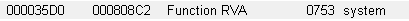
\includegraphics[width=10cm]{images/libc_system_rva.png}
	\caption{使用PEview查看msvcr120.dll的EXPORT Address Table}
	\label{fig:libc_system_rva}
\end{figure}

既然要以``cmd''为参数调用system()就要获得该字符串的地址。一种方法是直接将其嵌入shellcode,但这样就需要重定位,从而消耗更多的代码;本着shellcode的代码字节数越少越好的原则,这里选择另一种方法。可以在msvcr120.dll内找到字符串``cmd'',根据其RVA就可以获得实际地址。具体做法是,使用UltraEdit搜索之,然后在PEview中查看其RVA,如图\ref{fig:libc_cmd_rva}所示。

\begin{figure}[htbp]
	\centering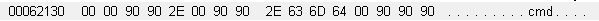
\includegraphics[width=12cm]{images/libc_cmd_rva.png}
	\caption{使用PEview查看msvcr120.dll的``cmd''字符串RVA}
	\label{fig:libc_cmd_rva}
\end{figure}

至此,已获得了system()和所需参数的地址,完成函数调用即可。

\subsection{shellcode的调整}
溢出攻击通常是基于strcpy()的漏洞,如果shellcode内包含0x00就会使得shellcode无法被完全拷贝,因此需要消除机器码中的0x00,比如``\# cmp eax, 0''和``\# mov eax, 1''之类指令就不能出现,应该使用等价指令例如``\# test eax, eax''和``\# xor eax, eax \# inc eax''进行替换。\par
还有一个关键问题,shellcode要完成模块msvcr120.dll的查找,此时就会涉及字符串的匹配,那么就需要把字符串``msvcr120.dll''嵌入shellcode,因此需要进行重定位。简单的重定位代码如下:

\begin{lstlisting}[language=C++, basicstyle=\ttfamily\tiny, numbers=left, numberstyle=\tiny, keywordstyle=\color{blue!70}, commentstyle=\color{red!50!green!50!blue!50}, frame=shadowbox, rulesepcolor=\color{red!20!green!20!blue!20}]
	CALL XXX;
XXX:
	POP EAX;
\end{lstlisting}

首先CALL指令将下一条指令的地址压栈,然后设置EIP为标号XXX的地址,于是就会执行``POP EAX'',而被CALL指令压栈的``下一条指令的地址''正好是标号XXX的实际地址(也就是``POP EAX''这条指令的实际地址),所以它就会被弹入EAX,shellcode就可以知道自己的实际地址,这就是EIP的自定位。但是这样的指令不能应用到shellcode中,因为``CALL XXX''的机器码是``E8 00 00 00 00''。为了实现EIP的自定位,可以使用如下的机器码:

\begin{lstlisting}[language=C++, basicstyle=\ttfamily\tiny, numbers=left, numberstyle=\tiny, keywordstyle=\color{blue!70}, commentstyle=\color{red!50!green!50!blue!50}, frame=shadowbox, rulesepcolor=\color{red!20!green!20!blue!20}]
CODE_ENTRY:
/* 0 */	 0xE8;
/* 1 */	 0xFF;
/* 2 */	 0xFF;
/* 3 */	 0xFF;
/* 4 */	 0xFF; // call 0xFFFFFFFF
LABEL_BASE:
/* 5 */	 0xC2;
/* 6 */	 0x59;
/* 7 */	 0x90;
\end{lstlisting}

``call -1''后LABEL\_BASE的地址被压栈, 然后eip指向标号4, 将标号4和5的``FFC2''译码成``inc edx''; 然后执行标号6的``pop ecx''(0x59), 将保存在栈顶的LABEL\_BASE的地址pop进ecx; 之后执行标号7的``nop''(0x90). 至此实现了自定位——LABEL\_BASE的地址被保存在ecx。

\section{突破数据执行保护(DEP}

\chapter{测试及分析}

\chapter{总结及展望}

\end{document}
